%\documentclass[unknownkeysallowed,usepdftitle=false]{beamer}
\documentclass[]{beamer}
% unknownkeysallowed is needed for mac and the newer latex version -> is more picky than before...
\usetheme{default}

\usepackage[utf8]{inputenc}
\usepackage{graphicx}
\usepackage{epsfig}
\usepackage{siunitx}
\usepackage{color}
\usepackage{ifthen}
\usepackage{ragged2e}
\usepackage{mwe}
\usepackage{multicol}
\usepackage{tikz}
\usetikzlibrary{positioning}
\usepackage[normalem]{ulem}

\usepackage{bm}
\usepackage{amsfonts}
\usepackage{amssymb}

\begin{document}
	\begin{frame}\frametitle{
	  	Biogeochemical Model Database  \texttt{bgc\_md2} 
	  }
	  \alert{Why would you want} a model data base?
	  \begin{itemize}
	  \item
	  	{\bf Find} (rather than reinvent) {\bf models} among {\bf many }:
		\\
		{\tiny 
		%(from A to Z):
	        Arora2005GCB-1 ,CARDAMOM ,$\dots$, Zelenev2000MicrobialEcology 
	        }
	  \item
		  {\bf Inspect} and {\bf compare} with common tools  
	          \begin{tabular}{lll}
	           % \resizebox{4cm}{!}{
	           \begin{minipage}{.3\textwidth}
	            	%\tiny
	            	\begin{align*}
	            	\frac{d}{dt}\left[\begin{matrix}leaf\\wood\end{matrix}\right] 
	            	=
	            	\left[
		    	    \begin{matrix}
		    	    	\dots
		    	    	\\
		    	    	\dots
		    	    \end{matrix}
		    	\right.
	            	\end{align*}
	            	\end{minipage}
	            %}
	            & 
		   \begin{minipage}{.3\textwidth}
			    \includegraphics[height=2cm]{Figures/7pool}
	            \end{minipage}
	            & 
	            \begin{minipage}{.3\textwidth}
			    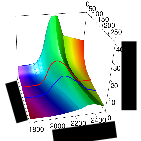
\includegraphics[height=2cm]{Figures/atmosphere_nonlinear}
	            \end{minipage}
		 	\\
		 	 	\centering{	{\bf symbolically 
				%\texttt{SymPy}
				}}
	         	 & 
		 	       \centering{	{\bf graphically} }
	         	 & 
		 	 	\centering{	{\bf numerically }}
	          %  $\dots$
	          \end{tabular}
	        %\end{itemize}
	  \item 
		  {\bf Use} common {\bf Infrastructure }\\
		  {\tiny python packages: \texttt{ComputabilityGraphs}, \texttt{CompartmentalSystems},  
		  100+ Unittests, Github CI, \texttt{Binder} \dots}
	
	  \item
		  {\bf Implement} new models {\bf in a day} with $\frac{1}{10}$ of the code
		  \\
		  {\tiny by reusing vs. reimplementing common functions, starting from examples vs. from scratch} 
	  \end{itemize}
	
	  \alert{Why not?} (Eager to listen to your ideas at the \alert{poster} ;-)
	  \\
	  \vspace{.5cm}
	  
\includegraphics[height=0.3cm, keepaspectratio]{Figures/bold_cornell_seal_cmyk_red}
	  \includegraphics[height=0.3cm, keepaspectratio]{Figures/minerva}
	  \includegraphics[height=0.3cm, keepaspectratio]{Figures/NAU}
	  \includegraphics[height=0.3cm, keepaspectratio]{Figures/idiv}
	  \includegraphics[height=0.3cm, keepaspectratio]{Figures/Logo_of_the_University_of_Melbourne}
	  \includegraphics[height=0.3cm, keepaspectratio]{Figures/EastChinaUni.png}
	  \includegraphics[height=0.3cm, keepaspectratio]{Figures/IGSNRR}
	  \includegraphics[height=0.3cm, keepaspectratio]{Figures/Northwest_A&F_University}
	  \includegraphics[height=0.3cm, keepaspectratio]{Figures/SLU}
	\end{frame}
\end{document}
